\documentclass[m3380-lec-main.tex]{subfiles}



\begin{document}

\chapter{Welcome to Algorithms and Python!}

\section*{Goals}
\begin{enumerate}[1.~]\setlength{\itemsep}{0pt}
\item Gain familiarity with the IDLE environment.
\item Learn some elementary Python syntax and commands.
\end{enumerate}

\section*{Special Instructions}
If you are using your own laptop, and did not follow the instructions posted on Blackboard, you will have to complete today's lecture on one of the University's computers and then download and install Python 3.5 yourself from \verb|http://python.org|.\bigskip

Please have IDLE open and running when you're reading notes so that you can actually work examples.\bigskip

We're going to extensively discuss actual Python code in these notes, so let me determine some conventions. If I write something like \verb|print|, you should understand that it is a Python command. Anything that looks like this:

\smallskip{\fn\begin{verbatim}
x=13
print(x**2)
\end{verbatim}
}\smallskip\noindent
is a piece of Python code.

%%%%%%%%%%%%%%%%%%%%%
\section{Interactive mode} When you first open IDLE, you should get a report like so:

\smallskip{\fn\begin{verbatim}
Python 3.5.0 (v3.5.0:374f501f4567, Sep 12 2015, 11:00:19) 
[GCC 4.2.1 (Apple Inc. build 5666) (dot 3)] on darwin
Type "copyright", "credits" or "license()" for more information.
>>> 
\end{verbatim}
}\smallskip\noindent

From this you can deduce two things: Python is running, and I use a Mac. The \verb|>>>| which appears at the bottom is the \emph{prompt}; it's waiting for you to give Python a command. For today's notes, I'll explicitly tell you when to press Return by showing \car.
\smallskip{\fn\begin{ipython}
\verb|>>> 3 + 7|\car\\
\verb|10|
\end{ipython}
}\smallskip\noindent
Congratulations, you've just used Python as a calculator! 

%%%%%%%%%%%%%%%%%%%%%

\section{Python and numbers}
Python works really well with integers (called \verb|int|s) and floating point numbers (called \verb|float|s), and carefully respects order of operations.
\smallskip{\fn\begin{ipython}
\verb|>>> 4 * (0 + 4 ** 2 - 1) / 3|\car\\
\verb|20.0|
\end{ipython}
}\smallskip\noindent
In the above example, we note two things: first, the \verb|**| operator is our power operator; second, we fed in all \verb|int|egers and the returned value was a \verb|float|. This is the behavior of \verb|/|, which is the division operator. Integer division (via the Division Algorithm) uses \verb|//| and \verb|%| for quotient and remainder respectively:
\smallskip{\fn\begin{ipython}
\verb|>>> 16 // 3|\car\\
\verb|5|\\
\verb|>>> 16 % 3|\car\\
\verb|1|
\end{ipython}
}\smallskip\noindent
To assign a value to a variable name, we use \verb|=|:
\smallskip{\fn\begin{ipython}
\verb|>>> spam = 5|\car\\
\verb|>>> eggs = spam|\car\\
\verb|>>> spam = 90.5|\car\\
\verb|>>> eggs|\car\\
\verb|5|\\
\verb|>>> spam|\car\\
\verb|90.5|
\end{ipython}
}\smallskip\noindent
We see now that first setting \verb|eggs| equal to the value of \verb|spam| and then changing \verb|spam| does not also change \verb|eggs|.
%%%%%%%%%%%%%%%%%%%%%

\section{Strings}
Mathematically, a \emph{string} is a finite sequence of symbols from an \emph{alphabet}, which is really just the set of allowable symbols. Python behaves similarly: if you can type something, it's an allowable symbol. Strings in Python are differentiated from variable names and commands by being enclosed in single or double quotes. The only difference between single and double quotes for Python has to do with quotes within strings.

The operation of attaching one string to the end of another string is called \emph{concatenation}, and is carried out in Python using the \verb|+| operator. Integer multiplication of strings produces multiple copies of the string.

\smallskip{\fn\begin{ipython}
\verb|>>> spam = 'There, he moved!'|\car\\
\verb|>>> eggs = "No he didn't, that was you hitting the cage!"|\car\\ \smallskip
\verb|>>> 3 * spam|\car\\\smallskip
\verb|'There, he moved!There, he moved!There, he moved!'|\\\smallskip
\verb|>>> spam + eggs|\car\\
\verb|"There, he moved!No he didn't, that was you hitting the cage!"|
\end{ipython}
}\smallskip\noindent
Observe that you must be careful when entering strings: improper use of quotation marks will cause syntax errors.

\smallskip{\fn\begin{ipython}
\verb|>>> eggs = 'No he didn't, that was you hitting the cage!'|\car\\
\verb|SyntaxError: invalid syntax|
\end{ipython}
}\smallskip\noindent
Another way to avoid this is to \emph{escape} the special character:

\smallskip{\fn\begin{ipython}
\verb|>>> eggs = 'No he didn\'t, that was you hitting the cage!'|\car\\
\verb|>>> eggs|\car \smallskip\\
\verb|"No he didn't, that was you hitting the cage!"|
\end{ipython}
}\smallskip\noindent
There are several other special ``escape characters," including \verb|\n| (new line) and \verb|\t| (tab) which will not display when a string is returned, but only when it is \verb|print|ed.

\smallskip{\fn\begin{ipython}{\fn
\verb|>>> eggs = 'No he didn\'t, that was you hitting the cage!\n\tI never!'|\car \\
\verb|>>> eggs|\car \\
\verb|"No he didn't, that was you hitting the cage!\n\tI never!"|\\
\verb|>>> print(eggs)|\car \smallskip\\
\verb|No he didn't, that was you hitting the cage!|\\ 
\verb|    I never!|
}\end{ipython}
}\smallskip\noindent
%
The \verb|print(...)| \emph{function} prints a formatted string version of whatever \emph{argument(s)} it is given; if it is given more than one argument, it separates them with a space:

\smallskip{\fn\begin{ipython}
\verb|>>> print(3, 5, spam)|\car \\
\verb|3 5 There, he moved!|
\end{ipython}
}\smallskip\noindent
The behavior of \verb|print| can be further controlled: if given the parameter \verb|sep='xx'| successive arguments would be separated by \verb|xx| rather than a space; if given the parameter \verb|end=' '| the string is terminated with a single space rather than a new line.

Since strings are actually sequences of printable characters, we should be able to access elements of the sequence individually; in other languages, these pieces are called \emph{characters}, but Python has no separate character class. They are simply strings of size 1. An extremely important thing to remember about Python is that all sequence-type objects have first index $0$. If you wanted to represent the sequence of positive integers less than or equal to 100,  $a=(1,2,3,4,\ldots, 100)$, the elements of the tuple would be $a_0=1$, $a_1=2$, $a_2=3$, and so on, up to $a_{99}=100$.

Rather than subscripts, indices in Python are given in square brackets. Trying to index a position outside a string will result in an error.

\smallskip{\fn\begin{ipython}
\verb|>>> spam = 'this is a string'|\car\\
\verb|>>> spam[0]|\car\\
\verb|'t'|\\
\verb|>>> spam[5]|\car\\
\verb|'i'|\\
\verb|>>> spam[-1]|\car\\
\verb|'g'|\\
\verb|>>> spam[42]|\car\\
\verb|Traceback (most recent call last):|\\
\verb|  File "<pyshell#36>", line 1, in <module>|\\
\verb|    spam[42]|\\
\verb|IndexError: string index out of range|
\end{ipython}
}\smallskip\noindent

\subsection{Slicing} You can access a substring by \emph{slicing} the string, but you have to be careful how slicing works. The best way to imagine it (as explained in the Python tutorial) is to think of the indices actually marking the dividers between letters in a string:
\[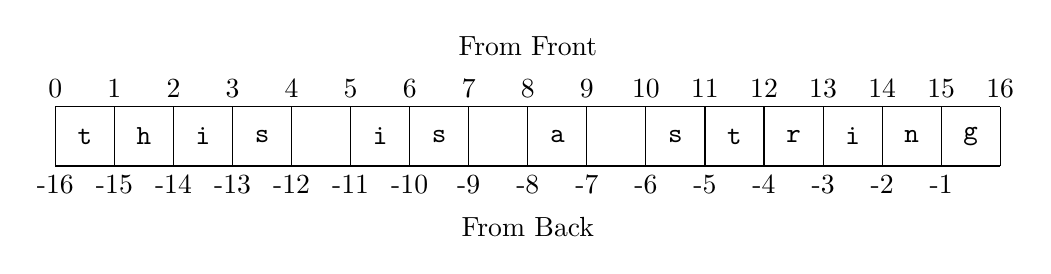
\begin{tikzpicture}[scale=.75]
\draw 
	(0,0) node [below] {-16} -- (16,0) 
	(16,1) node [above] {16} -- (0,1) node [above] {0};
\foreach \x in {0,1,...,16}{\draw (\x,0) -- (\x,1);}
\path
	(0.5,.5) node {\texttt{t}}
	(1.5,.5) node {\texttt{h}}
	(2.5,.5) node {\texttt{i}}
	(3.5,.5) node {\texttt{s}}
	(5.5,.5) node {\texttt{i}}
	(6.5,.5) node {\texttt{s}}
	(8.5,.5) node {\texttt{a}}
	(10.5,.5) node {\texttt{s}}
	(11.5,.5) node {\texttt{t}}
	(12.5,.5) node {\texttt{r}}
	(13.5,.5) node {\texttt{i}}
	(14.5,.5) node {\texttt{n}}
	(15.5,.5) node {\texttt{g}}
	(8,1.7) node [above] {From Front}
	(8,-.7) node [below] {From Back};
\foreach \x in {1,2,...,15}{
	\node [above] at (\x,1) {\x};
	\node [below] at (16-\x,0) {-\x};
}
\end{tikzpicture}\]

So if this is the string \verb|spam|, then we can see that \verb|spam[0]| gave us the single-letter string starting at index 0, and \verb|spam[-1]| gave us the single-letter string starting at index $-1$ from the back. If we want to isolate the word \verb|this| we can do it two ways. Since the word \verb|string| appears at the end of \verb|spam|, there are several ways to easily access it: 

\smallskip{\fn\begin{ipython}
\verb|>>> spam[0:4]|\car\\
\verb|'this'|\\
\verb|>>> spam[:4]|\car\\
\verb|'this'|\\
\verb|>>> spam[10:16]|\car\\
\verb|'string'|\\
\verb|>>> spam[10:]|\car\\
\verb|'string'|\\
\verb|>>> spam[-6:]|\car\\
\verb|'string'|
\end{ipython}
}\smallskip\noindent
Negative and positive indices can be mixed and matched, and mixing is handled smartly. Also, Python will accept a slice beyond the length of a string.

\smallskip{\fn\begin{ipython}
\verb|>>> spam[-11:9]|\car\\
\verb|'is a'|\\
\verb|>>> spam[8:-11]|\car\\
\verb|''|\\
\verb|>>> spam[8:42]|\car\\
\verb|'a string'|
\end{ipython}
}\smallskip\noindent
You can always find the length of your string using the \verb|len(...)| command:
\smallskip{\fn\begin{ipython}
\verb|>>> len(spam)|\car\\
\verb|16|
\end{ipython}
}\smallskip\noindent

\subsection{Strings are \emph{immutable}}
An important thing to note about strings is that you may read individual positions but you may not overwrite them.

\smallskip{\fn\begin{ipython}
\verb|>>> spam[5]='1'|\car\\
\verb|Traceback (most recent call last):|\\
\verb|  File "<pyshell#41>", line 1, in <module>|\\
\verb|    spam[5]='1'|\\
\verb|TypeError: 'str' object does not support item assignment|
\end{ipython}
}\smallskip\noindent

In the next lesson we will talk about other \emph{compound} objects which are \emph{mutable}, where you can change elements of the container one at a time.

\end{document}